\documentclass[12pt,a4paper]{article}
\usepackage[T1]{fontenc}
\usepackage[utf8]{inputenc}
\usepackage{amsmath,amssymb,amsfonts,amsthm,mathtools}
\usepackage{graphicx,float,geometry,hyperref,enumitem,xcolor}
\geometry{margin=2.5cm}

% Theorem environments
\theoremstyle{definition}
\newtheorem{definition}{Définition}[section]
\newtheorem{algorithme}{Algorithme}[section]
\theoremstyle{plain}
\newtheorem{theoreme}{Théorème}[section]
\newtheorem{proposition}{Proposition}[section]
\theoremstyle{remark}
\newtheorem{remarque}{Remarque}[section]
\newtheorem{invariants}{Invariants}[section]

% Macros
\newcommand{\tok}{\texttt{tok}}
\newcommand{\send}[2]{\mathrm{send}_{#1,#2}}
\newcommand{\recv}[2]{\mathrm{received}_{#1,#2}}
\newcommand{\cred}{\mathrm{cred}}
\newcommand{\ret}{\mathrm{ret}}

\title{\textbf{Cours 10 — Algorithmique Distribuée et Parallélisme}\\
\large Détection de terminaison \& Snapshot}
\date{25 mars 2026}
\author{}

\begin{document}
\maketitle
\tableofcontents
\newpage

% ─────────────────────────────────────────────────────────────────────────────
\section{Détection de terminaison — Algorithme de Safia (anneau)}
% ─────────────────────────────────────────────────────────────────────────────

Les processus $P_0, P_1, \ldots, P_{n-1}$ sont disposés en anneau.

\subsection{Variables locales du processus $p$}

\begin{itemize}
  \item $\mathrm{state} \in \{\text{actif}, \text{passif}\}$
  \item $\mathrm{color} \in \{\text{blanc}, \text{noir}\}$
  \item $\mathrm{me} \in \mathbb{Z}$, initialisé à $0$
\end{itemize}

\subsection{Comportement}

\paragraph{Quand $\mathrm{state} = \text{actif}$}
\begin{verbatim}
envoyer(message) ;
me := me + 1 ;
\end{verbatim}

\paragraph{Quand un message $\mathit{mes}$ arrive}
\begin{verbatim}
receive(mes) ;
me := me - 1 ;
color := noir ;
si état = actif alors état := passif ;
\end{verbatim}

\subsection{Lancement d'une détection de terminaison}

Le processus $P_0$ lance la détection en envoyant le jeton~:
\[
  \texttt{envoyer}(\tok,\,\text{blanc},\,0) \text{ à } P_{n-1}
\]

\subsection{Traitement du jeton $\langle \tok, c, q \rangle$ (quand $\mathrm{état} = \text{passif}$)}

\begin{algorithme}[Traitement du jeton — Safia]
\begin{verbatim}
si p = P_0 alors
    si (c = blanc) et (colorP = blanc) et (meP + q = 0)
    alors <Annoncer>
    sinon envoyer(tok, blanc, 0) à P_{n-1}
sinon
    si color = blanc
    alors envoyer(tok, c, q + meP) à suivant
    sinon envoyer(tok, noir, q + meP) à suivant ;
color := blanc ;
\end{verbatim}
\end{algorithme}

\begin{remarque}
Le jeton fait au plus 2 tours après la terminaison.
Référence~: Gerard Tel, \emph{Distributed Algorithms}, invariant de pupar.
\end{remarque}

% ─────────────────────────────────────────────────────────────────────────────
\section{Seconde version des compteurs — Algorithme de Mattern}
% ─────────────────────────────────────────────────────────────────────────────

Cette variante utilise un vecteur de compteurs~:
\[
  \begin{bmatrix} mc_1 \\ mc_2 \\ \vdots \\ mc_{n-1} \end{bmatrix}
\]
Le jeton fait au plus \textbf{1 tour} après la terminaison.

% ─────────────────────────────────────────────────────────────────────────────
\section{Algorithme du crédit — Mattern (calcul diffusant)}
% ─────────────────────────────────────────────────────────────────────────────

\subsection{Topologie et principe}

\begin{figure}[H]
  \centering
  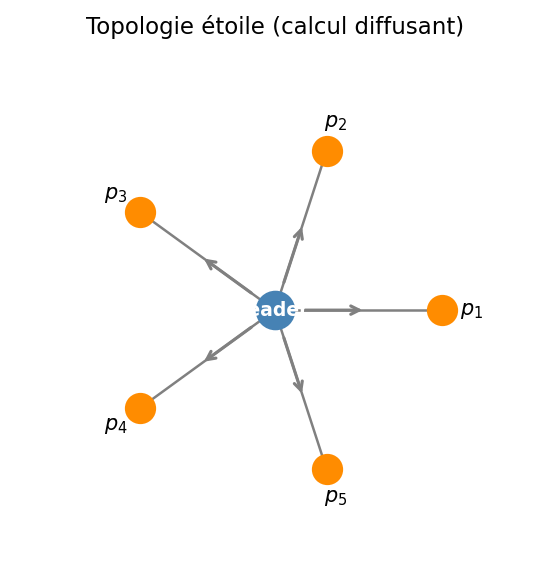
\includegraphics[width=0.46\textwidth]{figures/fig_leader_star.png}
  \caption{Topologie étoile~: le leader communique directement à chacun des processus.}
  \label{fig:leader_star}
\end{figure}

\begin{itemize}
  \item Quand le leader reçoit le signal de l'application, il positionne une variable $\mathrm{cr\acute{e}dit} = 1$.
  \item Tous les processus sont initialement passifs.
  \item Ils deviennent actifs par réception d'un message de travail du leader.
  \item Quand le leader envoie un message de travail au processus $p$, il joint le réel $\tfrac{1}{2}$ et conserve un crédit $\tfrac{1}{2}$.
  \item Quand un processus $p$ avec un crédit $c_p$ envoie un message à $q$, il attache $\tfrac{c_p}{2}$ au message et conserve $\tfrac{c_p}{2}$.
  \item Quand un processus avec un crédit $c_p$ reçoit un message transportant un crédit $c$, il fait $c_p \mathrel{:=} c_p + c$.
  \item Quand un processus devient passif, il renvoie son crédit au leader.
  \item Le leader a une variable $\ret$, initialisée à $0$; quand $\ret = 1$, il annonce la terminaison.
\end{itemize}

\subsection{Invariants}

\begin{invariants}
\begin{enumerate}
  \item La somme de tous les crédits (messages et processus) est égale à $1$.
  \item Un message de travail a un crédit strictement positif.
  \item Un processus actif a un crédit strictement positif.
\end{enumerate}
\end{invariants}

\subsection{Pseudo-code}

Variables pour le processus $p$~:
\begin{itemize}
  \item $\mathrm{state}_p \in \{\text{actif},\text{passif}\}$, actif si $p = P_0$, passif sinon.
  \item $\cred_p \in \mathbb{Q}$, initialisé à $1$ si $p = P_0$, sinon $0$.
  \item $\ret \in \mathbb{Q}$, initialisé à $0$ \textit{(pour $P_0$ seulement)}.
\end{itemize}

\paragraph{Si $\mathrm{state} = \text{actif}$ (piggybacking)}
\begin{verbatim}
envoyer(mes, cred/2) ;
cred := cred/2 ;
\end{verbatim}

\paragraph{Quand un message $(\mathit{mes}, c)$ arrive à $p$}
\begin{verbatim}
recevoir(mes, p) ;
state_p := actif ;
cred_p := cred_p + c ;
\end{verbatim}

\paragraph{Quand l'état de $p$ passe d'actif à passif}
\begin{verbatim}
envoyer(ret, cred_p) à P_0 ;
cred_p := 0 ;
\end{verbatim}

\paragraph{Quand un message $\ret$ arrive à $P_0$}
\begin{verbatim}
recevoir(ret, c) ;
ret := ret + c ;
si ret = 1 alors <Annoncer> ;
\end{verbatim}

\begin{remarque}
\textbf{Preuves.}
\begin{itemize}
  \item \emph{Pas de fausse annonce (fairness)~:} si l'application n'est pas terminée,
        $P_0$ n'annonce pas la terminaison, car il y a au moins un processus actif ou un message de travail en transit, donc $\ret \neq 1$.
  \item \emph{Annonce correcte~:} si l'application est terminée, il n'y a aucun
        processus actif ni message de travail, donc la somme de tous les crédits rendus
        vaut $1$, i.e.\ $\ret = 1$.
\end{itemize}
\end{remarque}

% ─────────────────────────────────────────────────────────────────────────────
\section{Snapshot / Instantané / Prise d'état global}
% ─────────────────────────────────────────────────────────────────────────────

À un moment donné, l'état local de l'application est sauvegardé~: $s^*$.

Un \emph{snapshot} est un n-uplet $\langle s_1^*, s_2^*, \ldots \rangle$ correspondant à une \emph{configuration} du système.
L'objectif est la \textbf{détection d'une propriété stable} (terminaison, blocage, \ldots).

\begin{figure}[H]
  \centering
  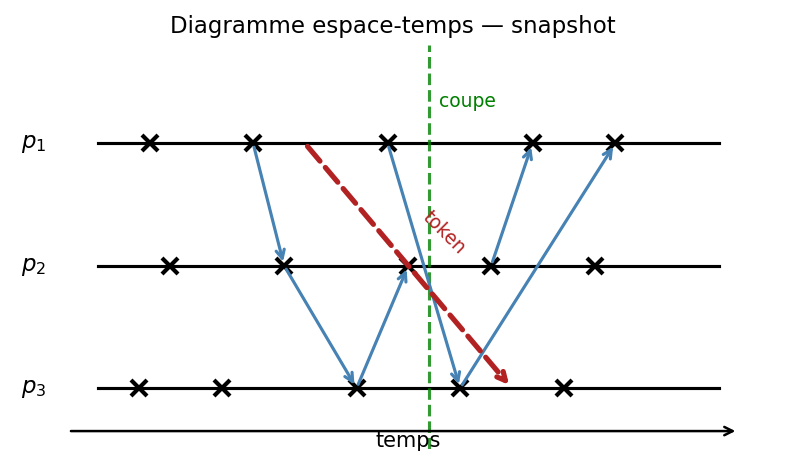
\includegraphics[width=0.72\textwidth]{figures/fig_spacetime_snapshot.png}
  \caption{Diagramme espace-temps illustrant la prise d'un snapshot (coupe verticale en pointillés verts).}
  \label{fig:snapshot_spacetime}
\end{figure}

\subsection{Hypothèse}

L'état d'un processus $p$ contient~:
\begin{itemize}
  \item $\send{p}{q}$ : la liste des messages émis vers le processus $q$, depuis le début de l'exécution.
  \item $\recv{q}{p}$ : la liste des messages reçus du processus $q$, depuis le début de l'exécution.
\end{itemize}

\begin{figure}[H]
  \centering
  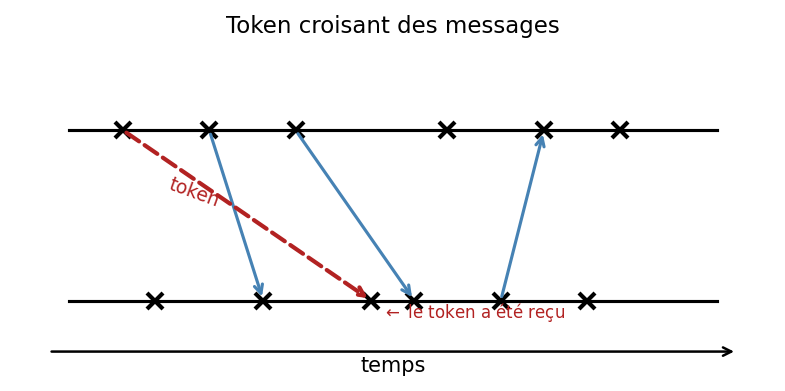
\includegraphics[width=0.70\textwidth]{figures/fig_token_crossing.png}
  \caption{Token croisant des messages en transit~: la réception du token indique le moment de la prise de snapshot.}
  \label{fig:token_crossing}
\end{figure}

\subsection{Définitions}

\begin{definition}[Snapshot possible]
Un snapshot est \emph{possible} si et seulement si pour tout processus $p$ et $q$~:
\[
  \send{p}{q} \subseteq \recv{q}{p}
\]
c'est-à-dire que l'ensemble des messages envoyés de $p$ à $q$ est inclus dans
l'ensemble des messages reçus par $q$ de $p$.
(Le schéma où un message est envoyé en pré-shot mais reçu en post-shot ne peut pas se produire.)
\end{definition}

\begin{definition}[Coupe cohérente]
Une \emph{coupe cohérente} est un ensemble d'événements clos par la relation de causalité $(\alpha_p)$.
La relation d'ordre $L_1 \preceq L_2$ est telle qu'un snapshot correspond à une coupe maximale pour l'inclusion~:
\begin{itemize}
  \item les éléments \emph{pré-shot} sont dans la coupe,
  \item les autres éléments sont \emph{post-shot}.
\end{itemize}
\end{definition}

\begin{definition}[Snapshot significatif]
Un snapshot est \emph{significatif} si la configuration $C^*$ peut être atteinte par une exécution.
\end{definition}

\subsection{Preuve de (1)+(2)+(3)}

On va prouver que $S^*$ est un snapshot possible, une coupe cohérente, et significatif.

Soient $e$ et $e'$ deux événements tels que $e \to e'$ (i.e.\ $e'$ est la réception d'un message émis lors de $e$).
On doit montrer que si $e'$ est pré-shot, alors $e$ est pré-shot.

On suit une exécution qui peut atteindre $S^*$.
Tout message pré-shot est reçu dans un événement pré-shot.

\begin{figure}[H]
  \centering
  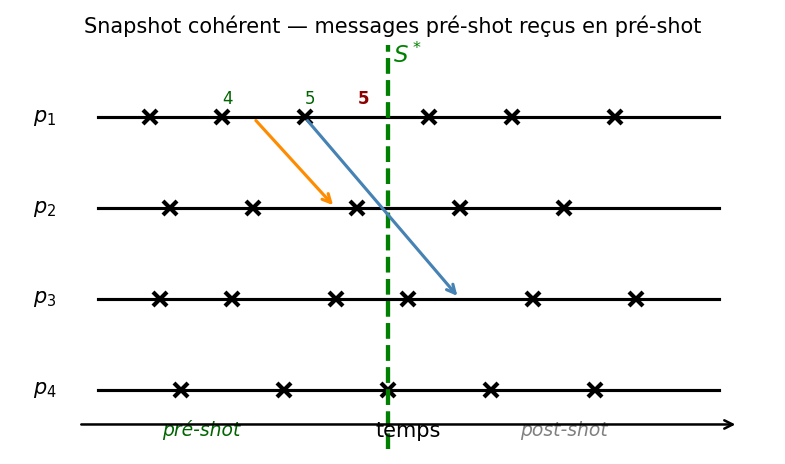
\includegraphics[width=0.78\textwidth]{figures/fig_preshot_postshot.png}
  \caption{Tout message pré-shot (avant la coupe $S^*$) est reçu dans un événement pré-shot.
           Un message traversant la coupe (bleu) aurait un envoi pré-shot et une réception post-shot~:
           c'est exactement ce qu'interdit la définition de snapshot cohérent.}
  \label{fig:preshot}
\end{figure}

\end{document}
